% Options for packages loaded elsewhere
\PassOptionsToPackage{unicode}{hyperref}
\PassOptionsToPackage{hyphens}{url}
%
\documentclass[
]{article}
\usepackage{lmodern}
\usepackage{amsmath}
\usepackage{ifxetex,ifluatex}
\ifnum 0\ifxetex 1\fi\ifluatex 1\fi=0 % if pdftex
  \usepackage[T1]{fontenc}
  \usepackage[utf8]{inputenc}
  \usepackage{textcomp} % provide euro and other symbols
  \usepackage{amssymb}
\else % if luatex or xetex
  \usepackage{unicode-math}
  \defaultfontfeatures{Scale=MatchLowercase}
  \defaultfontfeatures[\rmfamily]{Ligatures=TeX,Scale=1}
\fi
% Use upquote if available, for straight quotes in verbatim environments
\IfFileExists{upquote.sty}{\usepackage{upquote}}{}
\IfFileExists{microtype.sty}{% use microtype if available
  \usepackage[]{microtype}
  \UseMicrotypeSet[protrusion]{basicmath} % disable protrusion for tt fonts
}{}
\makeatletter
\@ifundefined{KOMAClassName}{% if non-KOMA class
  \IfFileExists{parskip.sty}{%
    \usepackage{parskip}
  }{% else
    \setlength{\parindent}{0pt}
    \setlength{\parskip}{6pt plus 2pt minus 1pt}}
}{% if KOMA class
  \KOMAoptions{parskip=half}}
\makeatother
\usepackage{xcolor}
\IfFileExists{xurl.sty}{\usepackage{xurl}}{} % add URL line breaks if available
\IfFileExists{bookmark.sty}{\usepackage{bookmark}}{\usepackage{hyperref}}
\hypersetup{
  pdftitle={5 - Transformation},
  hidelinks,
  pdfcreator={LaTeX via pandoc}}
\urlstyle{same} % disable monospaced font for URLs
\usepackage[margin=1in]{geometry}
\usepackage{color}
\usepackage{fancyvrb}
\newcommand{\VerbBar}{|}
\newcommand{\VERB}{\Verb[commandchars=\\\{\}]}
\DefineVerbatimEnvironment{Highlighting}{Verbatim}{commandchars=\\\{\}}
% Add ',fontsize=\small' for more characters per line
\usepackage{framed}
\definecolor{shadecolor}{RGB}{248,248,248}
\newenvironment{Shaded}{\begin{snugshade}}{\end{snugshade}}
\newcommand{\AlertTok}[1]{\textcolor[rgb]{0.94,0.16,0.16}{#1}}
\newcommand{\AnnotationTok}[1]{\textcolor[rgb]{0.56,0.35,0.01}{\textbf{\textit{#1}}}}
\newcommand{\AttributeTok}[1]{\textcolor[rgb]{0.77,0.63,0.00}{#1}}
\newcommand{\BaseNTok}[1]{\textcolor[rgb]{0.00,0.00,0.81}{#1}}
\newcommand{\BuiltInTok}[1]{#1}
\newcommand{\CharTok}[1]{\textcolor[rgb]{0.31,0.60,0.02}{#1}}
\newcommand{\CommentTok}[1]{\textcolor[rgb]{0.56,0.35,0.01}{\textit{#1}}}
\newcommand{\CommentVarTok}[1]{\textcolor[rgb]{0.56,0.35,0.01}{\textbf{\textit{#1}}}}
\newcommand{\ConstantTok}[1]{\textcolor[rgb]{0.00,0.00,0.00}{#1}}
\newcommand{\ControlFlowTok}[1]{\textcolor[rgb]{0.13,0.29,0.53}{\textbf{#1}}}
\newcommand{\DataTypeTok}[1]{\textcolor[rgb]{0.13,0.29,0.53}{#1}}
\newcommand{\DecValTok}[1]{\textcolor[rgb]{0.00,0.00,0.81}{#1}}
\newcommand{\DocumentationTok}[1]{\textcolor[rgb]{0.56,0.35,0.01}{\textbf{\textit{#1}}}}
\newcommand{\ErrorTok}[1]{\textcolor[rgb]{0.64,0.00,0.00}{\textbf{#1}}}
\newcommand{\ExtensionTok}[1]{#1}
\newcommand{\FloatTok}[1]{\textcolor[rgb]{0.00,0.00,0.81}{#1}}
\newcommand{\FunctionTok}[1]{\textcolor[rgb]{0.00,0.00,0.00}{#1}}
\newcommand{\ImportTok}[1]{#1}
\newcommand{\InformationTok}[1]{\textcolor[rgb]{0.56,0.35,0.01}{\textbf{\textit{#1}}}}
\newcommand{\KeywordTok}[1]{\textcolor[rgb]{0.13,0.29,0.53}{\textbf{#1}}}
\newcommand{\NormalTok}[1]{#1}
\newcommand{\OperatorTok}[1]{\textcolor[rgb]{0.81,0.36,0.00}{\textbf{#1}}}
\newcommand{\OtherTok}[1]{\textcolor[rgb]{0.56,0.35,0.01}{#1}}
\newcommand{\PreprocessorTok}[1]{\textcolor[rgb]{0.56,0.35,0.01}{\textit{#1}}}
\newcommand{\RegionMarkerTok}[1]{#1}
\newcommand{\SpecialCharTok}[1]{\textcolor[rgb]{0.00,0.00,0.00}{#1}}
\newcommand{\SpecialStringTok}[1]{\textcolor[rgb]{0.31,0.60,0.02}{#1}}
\newcommand{\StringTok}[1]{\textcolor[rgb]{0.31,0.60,0.02}{#1}}
\newcommand{\VariableTok}[1]{\textcolor[rgb]{0.00,0.00,0.00}{#1}}
\newcommand{\VerbatimStringTok}[1]{\textcolor[rgb]{0.31,0.60,0.02}{#1}}
\newcommand{\WarningTok}[1]{\textcolor[rgb]{0.56,0.35,0.01}{\textbf{\textit{#1}}}}
\usepackage{graphicx}
\makeatletter
\def\maxwidth{\ifdim\Gin@nat@width>\linewidth\linewidth\else\Gin@nat@width\fi}
\def\maxheight{\ifdim\Gin@nat@height>\textheight\textheight\else\Gin@nat@height\fi}
\makeatother
% Scale images if necessary, so that they will not overflow the page
% margins by default, and it is still possible to overwrite the defaults
% using explicit options in \includegraphics[width, height, ...]{}
\setkeys{Gin}{width=\maxwidth,height=\maxheight,keepaspectratio}
% Set default figure placement to htbp
\makeatletter
\def\fps@figure{htbp}
\makeatother
\setlength{\emergencystretch}{3em} % prevent overfull lines
\providecommand{\tightlist}{%
  \setlength{\itemsep}{0pt}\setlength{\parskip}{0pt}}
\setcounter{secnumdepth}{-\maxdimen} % remove section numbering
\ifluatex
  \usepackage{selnolig}  % disable illegal ligatures
\fi

\title{5 - Transformation}
\author{}
\date{\vspace{-2.5em}}

\begin{document}
\maketitle

\hypertarget{load-libraries-and-dataframe}{%
\subsubsection{Load libraries and
dataframe}\label{load-libraries-and-dataframe}}

\begin{Shaded}
\begin{Highlighting}[]
\FunctionTok{library}\NormalTok{(tidyverse)}
\FunctionTok{library}\NormalTok{(nycflights13)}
\FunctionTok{library}\NormalTok{(zoo) }\CommentTok{\# for computing running average}
\CommentTok{\#library(fitdistrplus) \#for beta distribution}
\end{Highlighting}
\end{Shaded}

\hypertarget{exercises}{%
\subsubsection{Exercises}\label{exercises}}

\begin{enumerate}
\def\labelenumi{\arabic{enumi}.}
\item
  Find all flights that
\item
  Had an arrival delay of two or more hours
\end{enumerate}

\begin{Shaded}
\begin{Highlighting}[]
\NormalTok{flights }\SpecialCharTok{\%\textgreater{}\%} \FunctionTok{filter}\NormalTok{(arr\_delay }\SpecialCharTok{\textgreater{}=} \DecValTok{120}\NormalTok{)}
\end{Highlighting}
\end{Shaded}

\begin{verbatim}
## # A tibble: 10,200 x 19
##     year month   day dep_time sched_dep_time dep_delay arr_time sched_arr_time
##    <int> <int> <int>    <int>          <int>     <dbl>    <int>          <int>
##  1  2013     1     1      811            630       101     1047            830
##  2  2013     1     1      848           1835       853     1001           1950
##  3  2013     1     1      957            733       144     1056            853
##  4  2013     1     1     1114            900       134     1447           1222
##  5  2013     1     1     1505           1310       115     1638           1431
##  6  2013     1     1     1525           1340       105     1831           1626
##  7  2013     1     1     1549           1445        64     1912           1656
##  8  2013     1     1     1558           1359       119     1718           1515
##  9  2013     1     1     1732           1630        62     2028           1825
## 10  2013     1     1     1803           1620       103     2008           1750
## # ... with 10,190 more rows, and 11 more variables: arr_delay <dbl>,
## #   carrier <chr>, flight <int>, tailnum <chr>, origin <chr>, dest <chr>,
## #   air_time <dbl>, distance <dbl>, hour <dbl>, minute <dbl>, time_hour <dttm>
\end{verbatim}

\begin{enumerate}
\def\labelenumi{\arabic{enumi}.}
\setcounter{enumi}{1}
\tightlist
\item
  Flew to Houston (\texttt{IAH} or \texttt{HOU})
\end{enumerate}

\begin{Shaded}
\begin{Highlighting}[]
\NormalTok{flights }\SpecialCharTok{\%\textgreater{}\%} \FunctionTok{filter}\NormalTok{(dest }\SpecialCharTok{\%in\%} \FunctionTok{c}\NormalTok{(}\StringTok{"IAH"}\NormalTok{, }\StringTok{"HOU"}\NormalTok{))}
\end{Highlighting}
\end{Shaded}

\begin{verbatim}
## # A tibble: 9,313 x 19
##     year month   day dep_time sched_dep_time dep_delay arr_time sched_arr_time
##    <int> <int> <int>    <int>          <int>     <dbl>    <int>          <int>
##  1  2013     1     1      517            515         2      830            819
##  2  2013     1     1      533            529         4      850            830
##  3  2013     1     1      623            627        -4      933            932
##  4  2013     1     1      728            732        -4     1041           1038
##  5  2013     1     1      739            739         0     1104           1038
##  6  2013     1     1      908            908         0     1228           1219
##  7  2013     1     1     1028           1026         2     1350           1339
##  8  2013     1     1     1044           1045        -1     1352           1351
##  9  2013     1     1     1114            900       134     1447           1222
## 10  2013     1     1     1205           1200         5     1503           1505
## # ... with 9,303 more rows, and 11 more variables: arr_delay <dbl>,
## #   carrier <chr>, flight <int>, tailnum <chr>, origin <chr>, dest <chr>,
## #   air_time <dbl>, distance <dbl>, hour <dbl>, minute <dbl>, time_hour <dttm>
\end{verbatim}

\begin{enumerate}
\def\labelenumi{\arabic{enumi}.}
\setcounter{enumi}{2}
\tightlist
\item
  Were operated by United, American, or Delta First we have to check
  which code has each airline
\end{enumerate}

\begin{Shaded}
\begin{Highlighting}[]
\NormalTok{airlines}
\end{Highlighting}
\end{Shaded}

\begin{verbatim}
## # A tibble: 16 x 2
##    carrier name                       
##    <chr>   <chr>                      
##  1 9E      Endeavor Air Inc.          
##  2 AA      American Airlines Inc.     
##  3 AS      Alaska Airlines Inc.       
##  4 B6      JetBlue Airways            
##  5 DL      Delta Air Lines Inc.       
##  6 EV      ExpressJet Airlines Inc.   
##  7 F9      Frontier Airlines Inc.     
##  8 FL      AirTran Airways Corporation
##  9 HA      Hawaiian Airlines Inc.     
## 10 MQ      Envoy Air                  
## 11 OO      SkyWest Airlines Inc.      
## 12 UA      United Air Lines Inc.      
## 13 US      US Airways Inc.            
## 14 VX      Virgin America             
## 15 WN      Southwest Airlines Co.     
## 16 YV      Mesa Airlines Inc.
\end{verbatim}

Then we can filter for them

\begin{Shaded}
\begin{Highlighting}[]
\NormalTok{flights }\SpecialCharTok{\%\textgreater{}\%} \FunctionTok{filter}\NormalTok{(carrier }\SpecialCharTok{\%in\%} \FunctionTok{c}\NormalTok{(}\StringTok{"DL"}\NormalTok{, }\StringTok{"AA"}\NormalTok{, }\StringTok{"UA"}\NormalTok{))}
\end{Highlighting}
\end{Shaded}

\begin{verbatim}
## # A tibble: 139,504 x 19
##     year month   day dep_time sched_dep_time dep_delay arr_time sched_arr_time
##    <int> <int> <int>    <int>          <int>     <dbl>    <int>          <int>
##  1  2013     1     1      517            515         2      830            819
##  2  2013     1     1      533            529         4      850            830
##  3  2013     1     1      542            540         2      923            850
##  4  2013     1     1      554            600        -6      812            837
##  5  2013     1     1      554            558        -4      740            728
##  6  2013     1     1      558            600        -2      753            745
##  7  2013     1     1      558            600        -2      924            917
##  8  2013     1     1      558            600        -2      923            937
##  9  2013     1     1      559            600        -1      941            910
## 10  2013     1     1      559            600        -1      854            902
## # ... with 139,494 more rows, and 11 more variables: arr_delay <dbl>,
## #   carrier <chr>, flight <int>, tailnum <chr>, origin <chr>, dest <chr>,
## #   air_time <dbl>, distance <dbl>, hour <dbl>, minute <dbl>, time_hour <dttm>
\end{verbatim}

\begin{enumerate}
\def\labelenumi{\arabic{enumi}.}
\setcounter{enumi}{3}
\tightlist
\item
  Departed in summer (July, August, and September)
\end{enumerate}

\begin{Shaded}
\begin{Highlighting}[]
\NormalTok{flights }\SpecialCharTok{\%\textgreater{}\%} \FunctionTok{filter}\NormalTok{(month }\SpecialCharTok{\%in\%} \DecValTok{7}\SpecialCharTok{:}\DecValTok{9}\NormalTok{)}
\end{Highlighting}
\end{Shaded}

\begin{verbatim}
## # A tibble: 86,326 x 19
##     year month   day dep_time sched_dep_time dep_delay arr_time sched_arr_time
##    <int> <int> <int>    <int>          <int>     <dbl>    <int>          <int>
##  1  2013     7     1        1           2029       212      236           2359
##  2  2013     7     1        2           2359         3      344            344
##  3  2013     7     1       29           2245       104      151              1
##  4  2013     7     1       43           2130       193      322             14
##  5  2013     7     1       44           2150       174      300            100
##  6  2013     7     1       46           2051       235      304           2358
##  7  2013     7     1       48           2001       287      308           2305
##  8  2013     7     1       58           2155       183      335             43
##  9  2013     7     1      100           2146       194      327             30
## 10  2013     7     1      100           2245       135      337            135
## # ... with 86,316 more rows, and 11 more variables: arr_delay <dbl>,
## #   carrier <chr>, flight <int>, tailnum <chr>, origin <chr>, dest <chr>,
## #   air_time <dbl>, distance <dbl>, hour <dbl>, minute <dbl>, time_hour <dttm>
\end{verbatim}

\begin{enumerate}
\def\labelenumi{\arabic{enumi}.}
\setcounter{enumi}{4}
\tightlist
\item
  Arrived more than two hours late, but didn't leave late
\end{enumerate}

\begin{Shaded}
\begin{Highlighting}[]
\NormalTok{flights }\SpecialCharTok{\%\textgreater{}\%} \FunctionTok{filter}\NormalTok{(arr\_delay }\SpecialCharTok{\textgreater{}=} \DecValTok{120} \SpecialCharTok{\&}\NormalTok{ dep\_delay }\SpecialCharTok{\textless{}=} \DecValTok{0}\NormalTok{)}
\end{Highlighting}
\end{Shaded}

\begin{verbatim}
## # A tibble: 29 x 19
##     year month   day dep_time sched_dep_time dep_delay arr_time sched_arr_time
##    <int> <int> <int>    <int>          <int>     <dbl>    <int>          <int>
##  1  2013     1    27     1419           1420        -1     1754           1550
##  2  2013    10     7     1350           1350         0     1736           1526
##  3  2013    10     7     1357           1359        -2     1858           1654
##  4  2013    10    16      657            700        -3     1258           1056
##  5  2013    11     1      658            700        -2     1329           1015
##  6  2013     3    18     1844           1847        -3       39           2219
##  7  2013     4    17     1635           1640        -5     2049           1845
##  8  2013     4    18      558            600        -2     1149            850
##  9  2013     4    18      655            700        -5     1213            950
## 10  2013     5    22     1827           1830        -3     2217           2010
## # ... with 19 more rows, and 11 more variables: arr_delay <dbl>, carrier <chr>,
## #   flight <int>, tailnum <chr>, origin <chr>, dest <chr>, air_time <dbl>,
## #   distance <dbl>, hour <dbl>, minute <dbl>, time_hour <dttm>
\end{verbatim}

\begin{enumerate}
\def\labelenumi{\arabic{enumi}.}
\setcounter{enumi}{5}
\tightlist
\item
  Were delayed by at least an hour, but made up over 30 minutes in
  flight
\end{enumerate}

\begin{Shaded}
\begin{Highlighting}[]
\NormalTok{flights }\SpecialCharTok{\%\textgreater{}\%} \FunctionTok{filter}\NormalTok{(dep\_delay }\SpecialCharTok{\textgreater{}=} \DecValTok{60} \SpecialCharTok{\&}\NormalTok{ arr\_delay }\SpecialCharTok{\textless{}}\NormalTok{ dep\_delay }\SpecialCharTok{{-}} \DecValTok{30}\NormalTok{)}
\end{Highlighting}
\end{Shaded}

\begin{verbatim}
## # A tibble: 1,844 x 19
##     year month   day dep_time sched_dep_time dep_delay arr_time sched_arr_time
##    <int> <int> <int>    <int>          <int>     <dbl>    <int>          <int>
##  1  2013     1     1     2205           1720       285       46           2040
##  2  2013     1     1     2326           2130       116      131             18
##  3  2013     1     3     1503           1221       162     1803           1555
##  4  2013     1     3     1839           1700        99     2056           1950
##  5  2013     1     3     1850           1745        65     2148           2120
##  6  2013     1     3     1941           1759       102     2246           2139
##  7  2013     1     3     1950           1845        65     2228           2227
##  8  2013     1     3     2015           1915        60     2135           2111
##  9  2013     1     3     2257           2000       177       45           2224
## 10  2013     1     4     1917           1700       137     2135           1950
## # ... with 1,834 more rows, and 11 more variables: arr_delay <dbl>,
## #   carrier <chr>, flight <int>, tailnum <chr>, origin <chr>, dest <chr>,
## #   air_time <dbl>, distance <dbl>, hour <dbl>, minute <dbl>, time_hour <dttm>
\end{verbatim}

\begin{enumerate}
\def\labelenumi{\arabic{enumi}.}
\setcounter{enumi}{6}
\tightlist
\item
  Departed between midnight and 6am (inclusive)
\end{enumerate}

\begin{Shaded}
\begin{Highlighting}[]
\NormalTok{flights }\SpecialCharTok{\%\textgreater{}\%} \FunctionTok{filter}\NormalTok{(dep\_time }\SpecialCharTok{\%in\%} \DecValTok{0000}\SpecialCharTok{:}\DecValTok{0600}\NormalTok{)}
\end{Highlighting}
\end{Shaded}

\begin{verbatim}
## # A tibble: 9,344 x 19
##     year month   day dep_time sched_dep_time dep_delay arr_time sched_arr_time
##    <int> <int> <int>    <int>          <int>     <dbl>    <int>          <int>
##  1  2013     1     1      517            515         2      830            819
##  2  2013     1     1      533            529         4      850            830
##  3  2013     1     1      542            540         2      923            850
##  4  2013     1     1      544            545        -1     1004           1022
##  5  2013     1     1      554            600        -6      812            837
##  6  2013     1     1      554            558        -4      740            728
##  7  2013     1     1      555            600        -5      913            854
##  8  2013     1     1      557            600        -3      709            723
##  9  2013     1     1      557            600        -3      838            846
## 10  2013     1     1      558            600        -2      753            745
## # ... with 9,334 more rows, and 11 more variables: arr_delay <dbl>,
## #   carrier <chr>, flight <int>, tailnum <chr>, origin <chr>, dest <chr>,
## #   air_time <dbl>, distance <dbl>, hour <dbl>, minute <dbl>, time_hour <dttm>
\end{verbatim}

\begin{enumerate}
\def\labelenumi{\arabic{enumi}.}
\setcounter{enumi}{1}
\tightlist
\item
  Another useful dplyr filtering helper is \texttt{between()}. What does
  it do? Can you use it to simplify the code needed to answer the
  previous challenges?
\end{enumerate}

\begin{Shaded}
\begin{Highlighting}[]
\NormalTok{flights }\SpecialCharTok{\%\textgreater{}\%} \FunctionTok{filter}\NormalTok{(}\FunctionTok{between}\NormalTok{(month, }\DecValTok{7}\NormalTok{, }\DecValTok{9}\NormalTok{))}
\end{Highlighting}
\end{Shaded}

\begin{verbatim}
## # A tibble: 86,326 x 19
##     year month   day dep_time sched_dep_time dep_delay arr_time sched_arr_time
##    <int> <int> <int>    <int>          <int>     <dbl>    <int>          <int>
##  1  2013     7     1        1           2029       212      236           2359
##  2  2013     7     1        2           2359         3      344            344
##  3  2013     7     1       29           2245       104      151              1
##  4  2013     7     1       43           2130       193      322             14
##  5  2013     7     1       44           2150       174      300            100
##  6  2013     7     1       46           2051       235      304           2358
##  7  2013     7     1       48           2001       287      308           2305
##  8  2013     7     1       58           2155       183      335             43
##  9  2013     7     1      100           2146       194      327             30
## 10  2013     7     1      100           2245       135      337            135
## # ... with 86,316 more rows, and 11 more variables: arr_delay <dbl>,
## #   carrier <chr>, flight <int>, tailnum <chr>, origin <chr>, dest <chr>,
## #   air_time <dbl>, distance <dbl>, hour <dbl>, minute <dbl>, time_hour <dttm>
\end{verbatim}

\begin{Shaded}
\begin{Highlighting}[]
\NormalTok{flights }\SpecialCharTok{\%\textgreater{}\%} \FunctionTok{filter}\NormalTok{(}\FunctionTok{between}\NormalTok{(dep\_time, }\DecValTok{0000}\NormalTok{, }\DecValTok{0600}\NormalTok{))}
\end{Highlighting}
\end{Shaded}

\begin{verbatim}
## # A tibble: 9,344 x 19
##     year month   day dep_time sched_dep_time dep_delay arr_time sched_arr_time
##    <int> <int> <int>    <int>          <int>     <dbl>    <int>          <int>
##  1  2013     1     1      517            515         2      830            819
##  2  2013     1     1      533            529         4      850            830
##  3  2013     1     1      542            540         2      923            850
##  4  2013     1     1      544            545        -1     1004           1022
##  5  2013     1     1      554            600        -6      812            837
##  6  2013     1     1      554            558        -4      740            728
##  7  2013     1     1      555            600        -5      913            854
##  8  2013     1     1      557            600        -3      709            723
##  9  2013     1     1      557            600        -3      838            846
## 10  2013     1     1      558            600        -2      753            745
## # ... with 9,334 more rows, and 11 more variables: arr_delay <dbl>,
## #   carrier <chr>, flight <int>, tailnum <chr>, origin <chr>, dest <chr>,
## #   air_time <dbl>, distance <dbl>, hour <dbl>, minute <dbl>, time_hour <dttm>
\end{verbatim}

\begin{enumerate}
\def\labelenumi{\arabic{enumi}.}
\setcounter{enumi}{2}
\tightlist
\item
  How many flights have a missing \texttt{dep\_time}? What other
  variables are missing? What might these rows represent?
\end{enumerate}

\begin{Shaded}
\begin{Highlighting}[]
\NormalTok{flights }\SpecialCharTok{\%\textgreater{}\%} \FunctionTok{filter}\NormalTok{(}\FunctionTok{is.na}\NormalTok{(dep\_time))}
\end{Highlighting}
\end{Shaded}

\begin{verbatim}
## # A tibble: 8,255 x 19
##     year month   day dep_time sched_dep_time dep_delay arr_time sched_arr_time
##    <int> <int> <int>    <int>          <int>     <dbl>    <int>          <int>
##  1  2013     1     1       NA           1630        NA       NA           1815
##  2  2013     1     1       NA           1935        NA       NA           2240
##  3  2013     1     1       NA           1500        NA       NA           1825
##  4  2013     1     1       NA            600        NA       NA            901
##  5  2013     1     2       NA           1540        NA       NA           1747
##  6  2013     1     2       NA           1620        NA       NA           1746
##  7  2013     1     2       NA           1355        NA       NA           1459
##  8  2013     1     2       NA           1420        NA       NA           1644
##  9  2013     1     2       NA           1321        NA       NA           1536
## 10  2013     1     2       NA           1545        NA       NA           1910
## # ... with 8,245 more rows, and 11 more variables: arr_delay <dbl>,
## #   carrier <chr>, flight <int>, tailnum <chr>, origin <chr>, dest <chr>,
## #   air_time <dbl>, distance <dbl>, hour <dbl>, minute <dbl>, time_hour <dttm>
\end{verbatim}

\begin{verbatim}
8255 flights are missing dep_time.
Maybe they are cancelled flights, we can check if (missing dep_time - missing air_time) is empty to confirm this hypothesis.
\end{verbatim}

\begin{Shaded}
\begin{Highlighting}[]
\NormalTok{flights }\SpecialCharTok{\%\textgreater{}\%} \FunctionTok{filter}\NormalTok{(}\FunctionTok{is.na}\NormalTok{(dep\_time) }\SpecialCharTok{\&} \SpecialCharTok{!}\FunctionTok{is.na}\NormalTok{(air\_time))}
\end{Highlighting}
\end{Shaded}

\begin{verbatim}
## # A tibble: 0 x 19
## # ... with 19 variables: year <int>, month <int>, day <int>, dep_time <int>,
## #   sched_dep_time <int>, dep_delay <dbl>, arr_time <int>,
## #   sched_arr_time <int>, arr_delay <dbl>, carrier <chr>, flight <int>,
## #   tailnum <chr>, origin <chr>, dest <chr>, air_time <dbl>, distance <dbl>,
## #   hour <dbl>, minute <dbl>, time_hour <dttm>
\end{verbatim}

\begin{enumerate}
\def\labelenumi{\arabic{enumi}.}
\setcounter{enumi}{3}
\tightlist
\item
  Why is \texttt{NA\ \^{}\ 0} not missing?Why is
  \texttt{NA\ \textbar{}\ TRUE} not missing? Why is
  \texttt{FALSE\ \&\ NA} not missing? Can you figure out the general
  rule? (\texttt{NA\ *\ 0} is a tricky counterexample!)
\end{enumerate}

The NA could be any number. If the number is finite, then the result of
the multiplication will be 0, the exponential zero will be 1 and logical
operation will show that result under any circumstance.

Counterexample: However, if the the number is Inf, then the result of
the multiplication will be NaN. We don't know if the multiplication
results in 0 or NaN so the result is given as NA.

\hypertarget{exercises-1}{%
\subsubsection{Exercises}\label{exercises-1}}

\begin{enumerate}
\def\labelenumi{\arabic{enumi}.}
\tightlist
\item
  How could you use \texttt{arrange()} to sort all missing values to the
  start? (Hint: use \texttt{is.na()}).
\end{enumerate}

First we have to check where the NAs are

\begin{Shaded}
\begin{Highlighting}[]
\FunctionTok{sapply}\NormalTok{(flights, }\ControlFlowTok{function}\NormalTok{(x) }\FunctionTok{sum}\NormalTok{(}\FunctionTok{is.na}\NormalTok{(x)) )}
\end{Highlighting}
\end{Shaded}

\begin{verbatim}
##           year          month            day       dep_time sched_dep_time 
##              0              0              0           8255              0 
##      dep_delay       arr_time sched_arr_time      arr_delay        carrier 
##           8255           8713              0           9430              0 
##         flight        tailnum         origin           dest       air_time 
##              0           2512              0              0           9430 
##       distance           hour         minute      time_hour 
##              0              0              0              0
\end{verbatim}

Then for each column with NA we sort the dataset (the more NAs, the
higher is the position)

\begin{Shaded}
\begin{Highlighting}[]
\NormalTok{flights }\SpecialCharTok{\%\textgreater{}\%} \FunctionTok{arrange}\NormalTok{(}\FunctionTok{desc}\NormalTok{(}\FunctionTok{is.na}\NormalTok{(dep\_time) }\SpecialCharTok{+}
                         \FunctionTok{is.na}\NormalTok{(arr\_time) }\SpecialCharTok{+}
                         \FunctionTok{is.na}\NormalTok{(tailnum)  }\SpecialCharTok{+}
                         \FunctionTok{is.na}\NormalTok{(air\_time) ))}
\end{Highlighting}
\end{Shaded}

\begin{verbatim}
## # A tibble: 336,776 x 19
##     year month   day dep_time sched_dep_time dep_delay arr_time sched_arr_time
##    <int> <int> <int>    <int>          <int>     <dbl>    <int>          <int>
##  1  2013     1     2       NA           1545        NA       NA           1910
##  2  2013     1     2       NA           1601        NA       NA           1735
##  3  2013     1     3       NA            857        NA       NA           1209
##  4  2013     1     3       NA            645        NA       NA            952
##  5  2013     1     4       NA            845        NA       NA           1015
##  6  2013     1     4       NA           1830        NA       NA           2044
##  7  2013     1     5       NA            840        NA       NA           1001
##  8  2013     1     7       NA            820        NA       NA            958
##  9  2013     1     8       NA           1645        NA       NA           1838
## 10  2013     1     9       NA            755        NA       NA           1012
## # ... with 336,766 more rows, and 11 more variables: arr_delay <dbl>,
## #   carrier <chr>, flight <int>, tailnum <chr>, origin <chr>, dest <chr>,
## #   air_time <dbl>, distance <dbl>, hour <dbl>, minute <dbl>, time_hour <dttm>
\end{verbatim}

\begin{enumerate}
\def\labelenumi{\arabic{enumi}.}
\setcounter{enumi}{1}
\item
  Sort \texttt{flights} to find the most delayed flights. Find the
  flights that left earliest.

  {[}Note that earliest refers here to the absolute time and it is not
  compared to the sched\_dep\_time{]}
\end{enumerate}

\begin{Shaded}
\begin{Highlighting}[]
\FunctionTok{arrange}\NormalTok{(flights, }\FunctionTok{desc}\NormalTok{(dep\_delay), dep\_time)}
\end{Highlighting}
\end{Shaded}

\begin{verbatim}
## # A tibble: 336,776 x 19
##     year month   day dep_time sched_dep_time dep_delay arr_time sched_arr_time
##    <int> <int> <int>    <int>          <int>     <dbl>    <int>          <int>
##  1  2013     1     9      641            900      1301     1242           1530
##  2  2013     6    15     1432           1935      1137     1607           2120
##  3  2013     1    10     1121           1635      1126     1239           1810
##  4  2013     9    20     1139           1845      1014     1457           2210
##  5  2013     7    22      845           1600      1005     1044           1815
##  6  2013     4    10     1100           1900       960     1342           2211
##  7  2013     3    17     2321            810       911      135           1020
##  8  2013     6    27      959           1900       899     1236           2226
##  9  2013     7    22     2257            759       898      121           1026
## 10  2013    12     5      756           1700       896     1058           2020
## # ... with 336,766 more rows, and 11 more variables: arr_delay <dbl>,
## #   carrier <chr>, flight <int>, tailnum <chr>, origin <chr>, dest <chr>,
## #   air_time <dbl>, distance <dbl>, hour <dbl>, minute <dbl>, time_hour <dttm>
\end{verbatim}

\begin{enumerate}
\def\labelenumi{\arabic{enumi}.}
\setcounter{enumi}{2}
\tightlist
\item
  Sort \texttt{flights} to find the fastest (highest speed) flights.
\end{enumerate}

\begin{Shaded}
\begin{Highlighting}[]
\FunctionTok{arrange}\NormalTok{(flights, }\FunctionTok{desc}\NormalTok{( distance}\SpecialCharTok{/}\NormalTok{air\_time ))}
\end{Highlighting}
\end{Shaded}

\begin{verbatim}
## # A tibble: 336,776 x 19
##     year month   day dep_time sched_dep_time dep_delay arr_time sched_arr_time
##    <int> <int> <int>    <int>          <int>     <dbl>    <int>          <int>
##  1  2013     5    25     1709           1700         9     1923           1937
##  2  2013     7     2     1558           1513        45     1745           1719
##  3  2013     5    13     2040           2025        15     2225           2226
##  4  2013     3    23     1914           1910         4     2045           2043
##  5  2013     1    12     1559           1600        -1     1849           1917
##  6  2013    11    17      650            655        -5     1059           1150
##  7  2013     2    21     2355           2358        -3      412            438
##  8  2013    11    17      759            800        -1     1212           1255
##  9  2013    11    16     2003           1925        38       17             36
## 10  2013    11    16     2349           2359       -10      402            440
## # ... with 336,766 more rows, and 11 more variables: arr_delay <dbl>,
## #   carrier <chr>, flight <int>, tailnum <chr>, origin <chr>, dest <chr>,
## #   air_time <dbl>, distance <dbl>, hour <dbl>, minute <dbl>, time_hour <dttm>
\end{verbatim}

\begin{enumerate}
\def\labelenumi{\arabic{enumi}.}
\setcounter{enumi}{3}
\tightlist
\item
  Which flights travelled the farthest? Which travelled the shortest?
\end{enumerate}

Farthest flight

\begin{Shaded}
\begin{Highlighting}[]
\FunctionTok{arrange}\NormalTok{(flights, }\FunctionTok{desc}\NormalTok{(distance)) }\SpecialCharTok{\%\textgreater{}\%} \FunctionTok{head}\NormalTok{(}\DecValTok{1}\NormalTok{)}
\end{Highlighting}
\end{Shaded}

\begin{verbatim}
## # A tibble: 1 x 19
##    year month   day dep_time sched_dep_time dep_delay arr_time sched_arr_time
##   <int> <int> <int>    <int>          <int>     <dbl>    <int>          <int>
## 1  2013     1     1      857            900        -3     1516           1530
## # ... with 11 more variables: arr_delay <dbl>, carrier <chr>, flight <int>,
## #   tailnum <chr>, origin <chr>, dest <chr>, air_time <dbl>, distance <dbl>,
## #   hour <dbl>, minute <dbl>, time_hour <dttm>
\end{verbatim}

Shortest non cancelled flight (second row)

\begin{Shaded}
\begin{Highlighting}[]
\FunctionTok{arrange}\NormalTok{(flights, distance) }\SpecialCharTok{\%\textgreater{}\%} \FunctionTok{head}\NormalTok{(}\DecValTok{2}\NormalTok{)}
\end{Highlighting}
\end{Shaded}

\begin{verbatim}
## # A tibble: 2 x 19
##    year month   day dep_time sched_dep_time dep_delay arr_time sched_arr_time
##   <int> <int> <int>    <int>          <int>     <dbl>    <int>          <int>
## 1  2013     7    27       NA            106        NA       NA            245
## 2  2013     1     3     2127           2129        -2     2222           2224
## # ... with 11 more variables: arr_delay <dbl>, carrier <chr>, flight <int>,
## #   tailnum <chr>, origin <chr>, dest <chr>, air_time <dbl>, distance <dbl>,
## #   hour <dbl>, minute <dbl>, time_hour <dttm>
\end{verbatim}

\hypertarget{exercises-2}{%
\subsubsection{Exercises}\label{exercises-2}}

\begin{enumerate}
\def\labelenumi{\arabic{enumi}.}
\tightlist
\item
  Brainstorm as many ways as possible to select \texttt{dep\_time},
  \texttt{dep\_delay}, \texttt{arr\_time}, and \texttt{arr\_delay} from
  \texttt{flights}.
\end{enumerate}

\begin{Shaded}
\begin{Highlighting}[]
\NormalTok{flights }\SpecialCharTok{\%\textgreater{}\%} \FunctionTok{select}\NormalTok{(}\DecValTok{4}\NormalTok{, }\DecValTok{6}\NormalTok{, }\DecValTok{7}\NormalTok{, }\DecValTok{9}\NormalTok{)}
\end{Highlighting}
\end{Shaded}

\begin{verbatim}
## # A tibble: 336,776 x 4
##    dep_time dep_delay arr_time arr_delay
##       <int>     <dbl>    <int>     <dbl>
##  1      517         2      830        11
##  2      533         4      850        20
##  3      542         2      923        33
##  4      544        -1     1004       -18
##  5      554        -6      812       -25
##  6      554        -4      740        12
##  7      555        -5      913        19
##  8      557        -3      709       -14
##  9      557        -3      838        -8
## 10      558        -2      753         8
## # ... with 336,766 more rows
\end{verbatim}

\begin{Shaded}
\begin{Highlighting}[]
\NormalTok{flights }\SpecialCharTok{\%\textgreater{}\%} \FunctionTok{select}\NormalTok{(}\FunctionTok{starts\_with}\NormalTok{(}\StringTok{"dep\_"}\NormalTok{), }\FunctionTok{starts\_with}\NormalTok{(}\StringTok{"arr\_"}\NormalTok{))}
\end{Highlighting}
\end{Shaded}

\begin{verbatim}
## # A tibble: 336,776 x 4
##    dep_time dep_delay arr_time arr_delay
##       <int>     <dbl>    <int>     <dbl>
##  1      517         2      830        11
##  2      533         4      850        20
##  3      542         2      923        33
##  4      544        -1     1004       -18
##  5      554        -6      812       -25
##  6      554        -4      740        12
##  7      555        -5      913        19
##  8      557        -3      709       -14
##  9      557        -3      838        -8
## 10      558        -2      753         8
## # ... with 336,766 more rows
\end{verbatim}

\begin{Shaded}
\begin{Highlighting}[]
\NormalTok{flights }\SpecialCharTok{\%\textgreater{}\%} \FunctionTok{select}\NormalTok{(}\FunctionTok{starts\_with}\NormalTok{(}\StringTok{"dep\_"}\NormalTok{)}\SpecialCharTok{|} \FunctionTok{starts\_with}\NormalTok{(}\StringTok{"arr\_"}\NormalTok{))}
\end{Highlighting}
\end{Shaded}

\begin{verbatim}
## # A tibble: 336,776 x 4
##    dep_time dep_delay arr_time arr_delay
##       <int>     <dbl>    <int>     <dbl>
##  1      517         2      830        11
##  2      533         4      850        20
##  3      542         2      923        33
##  4      544        -1     1004       -18
##  5      554        -6      812       -25
##  6      554        -4      740        12
##  7      555        -5      913        19
##  8      557        -3      709       -14
##  9      557        -3      838        -8
## 10      558        -2      753         8
## # ... with 336,766 more rows
\end{verbatim}

\begin{Shaded}
\begin{Highlighting}[]
\NormalTok{flights }\SpecialCharTok{\%\textgreater{}\%} \FunctionTok{select}\NormalTok{( (}\FunctionTok{contains}\NormalTok{(}\StringTok{"time"}\NormalTok{) }\SpecialCharTok{|} \FunctionTok{contains}\NormalTok{(}\StringTok{"delay"}\NormalTok{) ) }\SpecialCharTok{\&}
\NormalTok{                    (}\FunctionTok{contains}\NormalTok{(}\StringTok{"dep"}\NormalTok{)  }\SpecialCharTok{|} \FunctionTok{contains}\NormalTok{(}\StringTok{"arr"}\NormalTok{)   ) }\SpecialCharTok{\&} 
                    \SpecialCharTok{!}\FunctionTok{contains}\NormalTok{(}\StringTok{"sched"}\NormalTok{)                      )}
\end{Highlighting}
\end{Shaded}

\begin{verbatim}
## # A tibble: 336,776 x 4
##    dep_time arr_time dep_delay arr_delay
##       <int>    <int>     <dbl>     <dbl>
##  1      517      830         2        11
##  2      533      850         4        20
##  3      542      923         2        33
##  4      544     1004        -1       -18
##  5      554      812        -6       -25
##  6      554      740        -4        12
##  7      555      913        -5        19
##  8      557      709        -3       -14
##  9      557      838        -3        -8
## 10      558      753        -2         8
## # ... with 336,766 more rows
\end{verbatim}

\begin{enumerate}
\def\labelenumi{\arabic{enumi}.}
\setcounter{enumi}{1}
\tightlist
\item
  What happens if you include the name of a variable multiple times in a
  \texttt{select()} call? It doesn't get replicated, as in
\end{enumerate}

\begin{Shaded}
\begin{Highlighting}[]
\NormalTok{flights }\SpecialCharTok{\%\textgreater{}\%} \FunctionTok{select}\NormalTok{(arr\_time, arr\_time, arr\_time)}
\end{Highlighting}
\end{Shaded}

\begin{verbatim}
## # A tibble: 336,776 x 1
##    arr_time
##       <int>
##  1      830
##  2      850
##  3      923
##  4     1004
##  5      812
##  6      740
##  7      913
##  8      709
##  9      838
## 10      753
## # ... with 336,766 more rows
\end{verbatim}

\begin{enumerate}
\def\labelenumi{\arabic{enumi}.}
\setcounter{enumi}{2}
\item
  What does the \texttt{any\_of()} function do? Why might it be helpful
  in conjunction with this vector?

  It selects all the variables apart from the ones in any\_of

\begin{Shaded}
\begin{Highlighting}[]
\NormalTok{vars }\OtherTok{\textless{}{-}} \FunctionTok{c}\NormalTok{(}\StringTok{"year"}\NormalTok{, }\StringTok{"month"}\NormalTok{, }\StringTok{"day"}\NormalTok{, }\StringTok{"dep\_delay"}\NormalTok{, }\StringTok{"arr\_delay"}\NormalTok{)}
\NormalTok{flights }\SpecialCharTok{\%\textgreater{}\%} \FunctionTok{select}\NormalTok{(}\FunctionTok{any\_of}\NormalTok{(vars))}
\end{Highlighting}
\end{Shaded}

\begin{verbatim}
## # A tibble: 336,776 x 5
##     year month   day dep_delay arr_delay
##    <int> <int> <int>     <dbl>     <dbl>
##  1  2013     1     1         2        11
##  2  2013     1     1         4        20
##  3  2013     1     1         2        33
##  4  2013     1     1        -1       -18
##  5  2013     1     1        -6       -25
##  6  2013     1     1        -4        12
##  7  2013     1     1        -5        19
##  8  2013     1     1        -3       -14
##  9  2013     1     1        -3        -8
## 10  2013     1     1        -2         8
## # ... with 336,766 more rows
\end{verbatim}
\item
  Does the result of running the following code surprise you? How do the
  select helpers deal with case by default? How can you change that
  default?
\end{enumerate}

`r contains(match, ignore.case = TRUE, vars = NULL)'

\begin{verbatim}
```r
select(flights, contains("TIME"))
```
\end{verbatim}

\begin{Shaded}
\begin{Highlighting}[]
    \FunctionTok{select}\NormalTok{(flights, }\FunctionTok{contains}\NormalTok{(}\StringTok{"TIME"}\NormalTok{, }\AttributeTok{ignore.case =} \ConstantTok{FALSE}\NormalTok{))}
\end{Highlighting}
\end{Shaded}

\begin{verbatim}
## # A tibble: 336,776 x 0
\end{verbatim}

\hypertarget{exercises-3}{%
\subsubsection{Exercises}\label{exercises-3}}

\begin{enumerate}
\def\labelenumi{\arabic{enumi}.}
\tightlist
\item
  Currently \texttt{dep\_time} and \texttt{sched\_dep\_time} are
  convenient to look at, but hard to compute with because they're not
  really continuous numbers. Convert them to a more convenient
  representation of number of minutes since midnight.
\end{enumerate}

\begin{Shaded}
\begin{Highlighting}[]
\NormalTok{flights }\OtherTok{\textless{}{-}}\NormalTok{ flights }\SpecialCharTok{\%\textgreater{}\%}
  \FunctionTok{mutate}\NormalTok{(}
    \AttributeTok{dep\_time\_min =} \DecValTok{60}\SpecialCharTok{*}\NormalTok{ dep\_time }\SpecialCharTok{\%/\%} \DecValTok{100} \SpecialCharTok{+}\NormalTok{ dep\_time }\SpecialCharTok{\%\%} \DecValTok{100}\NormalTok{,}
    \AttributeTok{arr\_time\_min =} \DecValTok{60}\SpecialCharTok{*}\NormalTok{ arr\_time }\SpecialCharTok{\%/\%} \DecValTok{100} \SpecialCharTok{+}\NormalTok{ arr\_time }\SpecialCharTok{\%\%} \DecValTok{100}\NormalTok{,}
    \AttributeTok{sched\_dep\_time\_min =} \DecValTok{60}\SpecialCharTok{*}\NormalTok{ sched\_dep\_time }\SpecialCharTok{\%/\%} \DecValTok{100} \SpecialCharTok{+}\NormalTok{ sched\_dep\_time }\SpecialCharTok{\%\%} \DecValTok{100}
\NormalTok{    )}
\end{Highlighting}
\end{Shaded}

\begin{enumerate}
\def\labelenumi{\arabic{enumi}.}
\tightlist
\item
  Compare \texttt{air\_time} with \texttt{arr\_time\ -\ dep\_time}. What
  do you expect to see? What do you see? What do you need to do to fix
  it?
\end{enumerate}

\begin{Shaded}
\begin{Highlighting}[]
\NormalTok{flights }\OtherTok{\textless{}{-}}\NormalTok{ flights }\SpecialCharTok{\%\textgreater{}\%}
  \FunctionTok{mutate}\NormalTok{( }\AttributeTok{flight\_difference =}\NormalTok{ air\_time }\SpecialCharTok{{-}}\NormalTok{ (arr\_time }\SpecialCharTok{{-}}\NormalTok{ dep\_time\_min))}

\FunctionTok{ggplot}\NormalTok{(flights) }\SpecialCharTok{+}
  \FunctionTok{geom\_density}\NormalTok{(}\FunctionTok{aes}\NormalTok{(flights}\SpecialCharTok{$}\NormalTok{flight\_difference))}
\end{Highlighting}
\end{Shaded}

\begin{verbatim}
## Warning: Use of `flights$flight_difference` is discouraged. Use
## `flight_difference` instead.
\end{verbatim}

\begin{verbatim}
## Warning: Removed 9430 rows containing non-finite values (stat_density).
\end{verbatim}

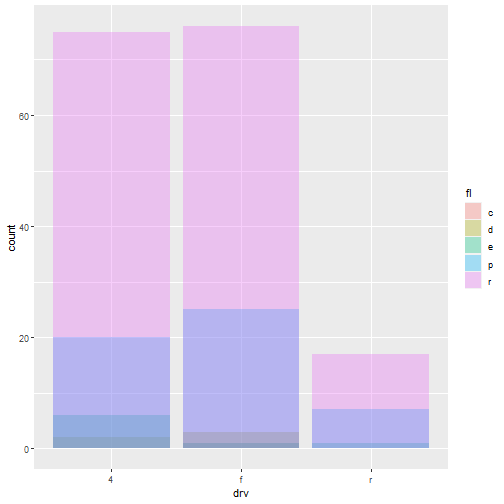
\includegraphics{5---Transformation_files/figure-latex/unnamed-chunk-26-1.pdf}

\begin{Shaded}
\begin{Highlighting}[]
\CommentTok{\# wrong}
\end{Highlighting}
\end{Shaded}

\begin{Shaded}
\begin{Highlighting}[]
\NormalTok{flights }\OtherTok{\textless{}{-}}\NormalTok{ flights }\SpecialCharTok{\%\textgreater{}\%}
  \FunctionTok{mutate}\NormalTok{( }\AttributeTok{flight\_difference\_min =}\NormalTok{ air\_time }\SpecialCharTok{{-}}\NormalTok{ (arr\_time\_min }\SpecialCharTok{{-}}\NormalTok{ dep\_time\_min))}

\FunctionTok{ggplot}\NormalTok{(flights) }\SpecialCharTok{+}
  \FunctionTok{geom\_density}\NormalTok{(}\FunctionTok{aes}\NormalTok{(flights}\SpecialCharTok{$}\NormalTok{flight\_difference\_min)) }\SpecialCharTok{+}
  \FunctionTok{geom\_vline}\NormalTok{(}\AttributeTok{xintercept =} \FunctionTok{c}\NormalTok{(}\DecValTok{60}\SpecialCharTok{*}\NormalTok{(}\SpecialCharTok{{-}}\DecValTok{2}\SpecialCharTok{:}\DecValTok{3}\NormalTok{)), }\AttributeTok{color =} \StringTok{"red"}\NormalTok{)}
\end{Highlighting}
\end{Shaded}

\begin{verbatim}
## Warning: Use of `flights$flight_difference_min` is discouraged. Use
## `flight_difference_min` instead.
\end{verbatim}

\begin{verbatim}
## Warning: Removed 9430 rows containing non-finite values (stat_density).
\end{verbatim}

\includegraphics{5---Transformation_files/figure-latex/unnamed-chunk-27-1.pdf}

There is the combined effect of time zones.

Moreover, the time now is calculated using minutes since midnight to
avoid effect of uncorrectly substract HHMM integers.

\begin{enumerate}
\def\labelenumi{\arabic{enumi}.}
\tightlist
\item
  Compare \texttt{dep\_time}, \texttt{sched\_dep\_time}, and
  \texttt{dep\_delay}. How would you expect those three numbers to be
  related?
\end{enumerate}

\begin{Shaded}
\begin{Highlighting}[]
\NormalTok{flights }\OtherTok{\textless{}{-}}\NormalTok{ flights }\SpecialCharTok{\%\textgreater{}\%}
  \FunctionTok{mutate}\NormalTok{( }\AttributeTok{dep\_difference =}\NormalTok{ dep\_delay }\SpecialCharTok{{-}}\NormalTok{ (dep\_time\_min }\SpecialCharTok{{-}}\NormalTok{ sched\_dep\_time\_min))}

\FunctionTok{ggplot}\NormalTok{(flights) }\SpecialCharTok{+}
  \FunctionTok{geom\_density}\NormalTok{(}\FunctionTok{aes}\NormalTok{(flights}\SpecialCharTok{$}\NormalTok{flight\_difference)) }\SpecialCharTok{+}
  \FunctionTok{geom\_vline}\NormalTok{(}\AttributeTok{xintercept =} \FunctionTok{median}\NormalTok{(flights}\SpecialCharTok{$}\NormalTok{flight\_difference, }\AttributeTok{na.rm =} \ConstantTok{TRUE}\NormalTok{),}
             \AttributeTok{color =} \StringTok{"red"}\NormalTok{)}
\end{Highlighting}
\end{Shaded}

\begin{verbatim}
## Warning: Use of `flights$flight_difference` is discouraged. Use
## `flight_difference` instead.
\end{verbatim}

\begin{verbatim}
## Warning: Removed 9430 rows containing non-finite values (stat_density).
\end{verbatim}

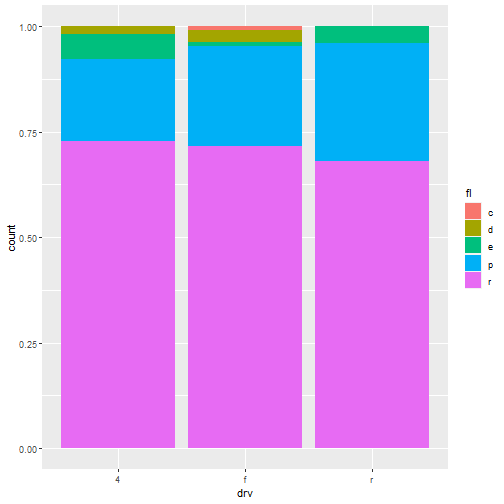
\includegraphics{5---Transformation_files/figure-latex/unnamed-chunk-28-1.pdf}

They should be related as
\texttt{dep\_delay\ =\ (dep\_time\ -\ sched\_dep\_time)}

\begin{enumerate}
\def\labelenumi{\arabic{enumi}.}
\tightlist
\item
  Find the 10 most delayed flights using a ranking function. How do you
  want to handle ties? Carefully read the documentation for
  \texttt{min\_rank()}.
\end{enumerate}

\begin{Shaded}
\begin{Highlighting}[]
\NormalTok{flights }\SpecialCharTok{\%\textgreater{}\%}
  \FunctionTok{select}\NormalTok{(flight, dep\_time\_min, sched\_dep\_time\_min) }\SpecialCharTok{\%\textgreater{}\%}
  \FunctionTok{mutate}\NormalTok{(}\AttributeTok{dep\_delay\_rank =} \FunctionTok{min\_rank}\NormalTok{(}\FunctionTok{desc}\NormalTok{(dep\_time\_min }\SpecialCharTok{{-}}\NormalTok{ sched\_dep\_time\_min))) }\SpecialCharTok{\%\textgreater{}\%}
  \FunctionTok{arrange}\NormalTok{(dep\_delay\_rank) }\SpecialCharTok{\%\textgreater{}\%}
  \FunctionTok{head}\NormalTok{(}\DecValTok{10}\NormalTok{)}
\end{Highlighting}
\end{Shaded}

\begin{verbatim}
## # A tibble: 10 x 4
##    flight dep_time_min sched_dep_time_min dep_delay_rank
##     <int>        <dbl>              <dbl>          <int>
##  1   2119         1401                490              1
##  2   2047         1377                479              2
##  3    835         1363                510              3
##  4   2319         1404                616              4
##  5    575         1161                375              5
##  6    502         1242                540              6
##  7    187         1283                630              7
##  8   1697         1381                745              8
##  9    411         1414                780              9
## 10     23         1259                630             10
\end{verbatim}

\begin{enumerate}
\def\labelenumi{\arabic{enumi}.}
\tightlist
\item
  What does \texttt{1:3\ +\ 1:10} return? Why?
\end{enumerate}

Error because longer object length is not a multiple of shorter object
length

\begin{enumerate}
\def\labelenumi{\arabic{enumi}.}
\tightlist
\item
  What trigonometric functions does R provide?
\end{enumerate}

cos(x), sin(x), tan(x), acos(x), asin(x), atan(x), atan2(y,x)

\hypertarget{exercises-4}{%
\subsubsection{Exercises}\label{exercises-4}}

\begin{enumerate}
\def\labelenumi{\arabic{enumi}.}
\item
  Brainstorm at least 5 different ways to assess the typical delay
  characteristics of a group of flights. Consider the following
  scenarios:

  \begin{itemize}
  \item
    A flight is 15 minutes early 50\% of the time, and 15 minutes late
    50\% of the time.
  \item
    A flight is always 10 minutes late.
  \item
    A flight is 30 minutes early 50\% of the time, and 30 minutes late
    50\% of the time.
  \item
    99\% of the time a flight is on time. 1\% of the time it's 2 hours
    late.
  \end{itemize}

  Which is more important: arrival delay or departure delay?
\end{enumerate}

It is more important the arrival delay.

Basic assessment involves median and average delay as well as variance
or IQR (filtering arr\_delay \textgreater{} 0), count and proportion of
flights with a no delay, small\_delay (\textless20') and significant
delay (\textgreater20').

geom\_dist can provide useful insights on delay pattern for that
particolar group.

\begin{Shaded}
\begin{Highlighting}[]
\NormalTok{flights }\SpecialCharTok{\%\textgreater{}\%}
  \FunctionTok{group\_by}\NormalTok{( carrier ) }\SpecialCharTok{\%\textgreater{}\%}
  \FunctionTok{summarize}\NormalTok{( }\AttributeTok{prop\_delay =} \FunctionTok{mean}\NormalTok{( arr\_delay }\SpecialCharTok{\textgreater{}} \DecValTok{0}\NormalTok{, }\AttributeTok{na.rm =} \ConstantTok{TRUE}\NormalTok{)) }
\end{Highlighting}
\end{Shaded}

\begin{verbatim}
## # A tibble: 16 x 2
##    carrier prop_delay
##  * <chr>        <dbl>
##  1 9E           0.384
##  2 AA           0.335
##  3 AS           0.267
##  4 B6           0.437
##  5 DL           0.344
##  6 EV           0.479
##  7 F9           0.576
##  8 FL           0.597
##  9 HA           0.284
## 10 MQ           0.467
## 11 OO           0.345
## 12 UA           0.385
## 13 US           0.371
## 14 VX           0.341
## 15 WN           0.440
## 16 YV           0.474
\end{verbatim}

\begin{Shaded}
\begin{Highlighting}[]
\NormalTok{flights }\SpecialCharTok{\%\textgreater{}\%}
  \FunctionTok{group\_by}\NormalTok{( carrier ) }\SpecialCharTok{\%\textgreater{}\%}
  \FunctionTok{filter}\NormalTok{ ( arr\_delay }\SpecialCharTok{\textgreater{}} \DecValTok{0}\NormalTok{ ) }\SpecialCharTok{\%\textgreater{}\%} 
  \FunctionTok{group\_by}\NormalTok{( carrier ) }\SpecialCharTok{\%\textgreater{}\%} 
  \FunctionTok{summarize}\NormalTok{( }\AttributeTok{mean\_delay =} \FunctionTok{mean}\NormalTok{(arr\_delay, }\AttributeTok{na.rm =} \ConstantTok{TRUE}\NormalTok{),}
             \AttributeTok{sd\_delay =} \FunctionTok{sd}\NormalTok{( arr\_delay, }\AttributeTok{na.rm =} \ConstantTok{TRUE}\NormalTok{),}
             \AttributeTok{median\_delay =} \FunctionTok{median}\NormalTok{( arr\_delay, }\AttributeTok{na.rm =} \ConstantTok{TRUE}\NormalTok{),}
             \AttributeTok{iqr\_delay =} \FunctionTok{IQR}\NormalTok{( arr\_delay, }\AttributeTok{na.rm =} \ConstantTok{TRUE}\NormalTok{)) }\SpecialCharTok{\%\textgreater{}\%} 
  \FunctionTok{arrange}\NormalTok{(}\FunctionTok{desc}\NormalTok{(mean\_delay))}
\end{Highlighting}
\end{Shaded}

\begin{verbatim}
## # A tibble: 16 x 5
##    carrier mean_delay sd_delay median_delay iqr_delay
##    <chr>        <dbl>    <dbl>        <dbl>     <dbl>
##  1 OO            60.6     56.7         47        86.2
##  2 YV            51.1     58.4         27.5      56.8
##  3 9E            49.3     58.9         27        57  
##  4 EV            48.3     55.4         28        56.2
##  5 F9            47.6     70.6         24        40.2
##  6 VX            43.8     65.4         17        44  
##  7 FL            41.1     61.4         19        38  
##  8 WN            40.7     55.9         19        40  
##  9 B6            40.0     49.2         22        44  
## 10 AA            38.3     54.3         19        39  
## 11 MQ            37.9     50.3         20        41  
## 12 DL            37.7     59.1         17        37  
## 13 UA            36.7     48.7         19        37  
## 14 HA            35.0    130.          14        18  
## 15 AS            34.4     41.6         17        34  
## 16 US            29.0     40.8         15        28
\end{verbatim}

\begin{Shaded}
\begin{Highlighting}[]
\FunctionTok{ggplot}\NormalTok{(}\FunctionTok{filter}\NormalTok{(flights, arr\_delay }\SpecialCharTok{\textgreater{}} \DecValTok{0}\NormalTok{)) }\SpecialCharTok{+}
  \FunctionTok{geom\_density}\NormalTok{( }\FunctionTok{aes}\NormalTok{( }\AttributeTok{x =}\NormalTok{ arr\_delay ), }\AttributeTok{color =} \StringTok{"grey50"}\NormalTok{, }\AttributeTok{size =} \DecValTok{2}\NormalTok{) }\SpecialCharTok{+}
  \FunctionTok{geom\_density}\NormalTok{( }\FunctionTok{aes}\NormalTok{( }\AttributeTok{x =}\NormalTok{ arr\_delay, }\AttributeTok{color =}\NormalTok{ carrier )) }\SpecialCharTok{+}
  \FunctionTok{scale\_x\_log10}\NormalTok{()}
\end{Highlighting}
\end{Shaded}

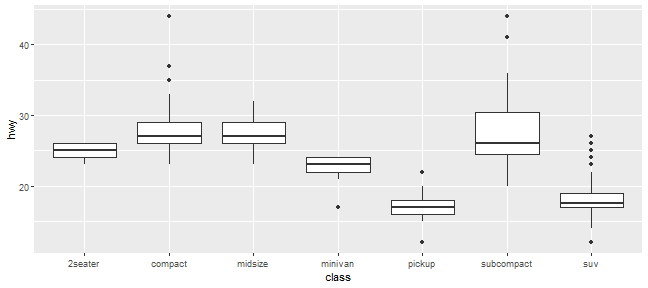
\includegraphics{5---Transformation_files/figure-latex/unnamed-chunk-32-1.pdf}

\begin{enumerate}
\def\labelenumi{\arabic{enumi}.}
\tightlist
\item
  Come up with another approach that will give you the same output as
  \texttt{not\_cancelled\ \%\textgreater{}\%\ count(dest)} and
  \texttt{not\_cancelled\ \%\textgreater{}\%\ count(tailnum,\ wt\ =\ distance)}
  (without using \texttt{count()}).
\end{enumerate}

\begin{Shaded}
\begin{Highlighting}[]
\NormalTok{not\_cancelled }\OtherTok{\textless{}{-}}\NormalTok{ flights }\SpecialCharTok{\%\textgreater{}\%} 
  \FunctionTok{filter}\NormalTok{(}\SpecialCharTok{!}\FunctionTok{is.na}\NormalTok{(dep\_delay), }\SpecialCharTok{!}\FunctionTok{is.na}\NormalTok{(arr\_delay))}

\NormalTok{not\_cancelled }\SpecialCharTok{\%\textgreater{}\%} 
  \FunctionTok{group\_by}\NormalTok{(dest) }\SpecialCharTok{\%\textgreater{}\%} 
  \FunctionTok{summarise}\NormalTok{( }\FunctionTok{n}\NormalTok{() )}
\end{Highlighting}
\end{Shaded}

\begin{verbatim}
## # A tibble: 104 x 2
##    dest  `n()`
##  * <chr> <int>
##  1 ABQ     254
##  2 ACK     264
##  3 ALB     418
##  4 ANC       8
##  5 ATL   16837
##  6 AUS    2411
##  7 AVL     261
##  8 BDL     412
##  9 BGR     358
## 10 BHM     269
## # ... with 94 more rows
\end{verbatim}

\begin{Shaded}
\begin{Highlighting}[]
\NormalTok{not\_cancelled }\SpecialCharTok{\%\textgreater{}\%} 
  \FunctionTok{group\_by}\NormalTok{(tailnum) }\SpecialCharTok{\%\textgreater{}\%} 
  \FunctionTok{summarise}\NormalTok{( }\FunctionTok{sum}\NormalTok{(distance) )}
\end{Highlighting}
\end{Shaded}

\begin{verbatim}
## # A tibble: 4,037 x 2
##    tailnum `sum(distance)`
##  * <chr>             <dbl>
##  1 D942DN             3418
##  2 N0EGMQ           239143
##  3 N10156           109664
##  4 N102UW            25722
##  5 N103US            24619
##  6 N104UW            24616
##  7 N10575           139903
##  8 N105UW            23618
##  9 N107US            21677
## 10 N108UW            32070
## # ... with 4,027 more rows
\end{verbatim}

\begin{enumerate}
\def\labelenumi{\arabic{enumi}.}
\tightlist
\item
  Our definition of cancelled flights
  (\texttt{is.na(dep\_delay)\ \textbar{}\ is.na(arr\_delay)} ) is
  slightly suboptimal. Why? Which is the most important column?
\end{enumerate}

We are interested only in arrived flights, which accounts also for
deviations or plane crashes

\begin{enumerate}
\def\labelenumi{\arabic{enumi}.}
\tightlist
\item
  Look at the number of cancelled flights per day. Is there a pattern?
  Is the proportion of cancelled flights related to the average delay?
\end{enumerate}

\begin{Shaded}
\begin{Highlighting}[]
\NormalTok{prop\_cancelled }\OtherTok{\textless{}{-}}\NormalTok{ flights }\SpecialCharTok{\%\textgreater{}\%} 
  \FunctionTok{group\_by}\NormalTok{( year, month, day ) }\SpecialCharTok{\%\textgreater{}\%} 
  \FunctionTok{summarise}\NormalTok{( }\AttributeTok{prop =} \FunctionTok{mean}\NormalTok{( }\FunctionTok{is.na}\NormalTok{(arr\_delay) ),}
             \AttributeTok{avg\_delay =} \FunctionTok{mean}\NormalTok{( arr\_delay[arr\_delay }\SpecialCharTok{\textgreater{}} \DecValTok{0}\NormalTok{], }\AttributeTok{na.rm =} \ConstantTok{TRUE}\NormalTok{ )) }\SpecialCharTok{\%\textgreater{}\%} 
  \FunctionTok{mutate}\NormalTok{( }\AttributeTok{date =} \FunctionTok{ISOdate}\NormalTok{(year, month, day) )}
\end{Highlighting}
\end{Shaded}

\begin{verbatim}
## `summarise()` has grouped output by 'year', 'month'. You can override using the `.groups` argument.
\end{verbatim}

\begin{Shaded}
\begin{Highlighting}[]
\FunctionTok{ggplot}\NormalTok{(prop\_cancelled) }\SpecialCharTok{+}
  \FunctionTok{geom\_col}\NormalTok{( }\FunctionTok{aes}\NormalTok{( }\AttributeTok{x =}\NormalTok{ date, }\AttributeTok{y =}\NormalTok{ prop, }\AttributeTok{fill =} \FunctionTok{weekdays}\NormalTok{(date))) }\SpecialCharTok{+}
  \FunctionTok{geom\_line}\NormalTok{(}\FunctionTok{aes}\NormalTok{( }\AttributeTok{x =}\NormalTok{ date, }\AttributeTok{y=}\FunctionTok{rollmean}\NormalTok{(prop, }\DecValTok{7}\NormalTok{, }\AttributeTok{fill =} \ConstantTok{NA}\NormalTok{))) }\SpecialCharTok{+}
  \FunctionTok{geom\_line}\NormalTok{(}\FunctionTok{aes}\NormalTok{( }\AttributeTok{x =}\NormalTok{ date, }\AttributeTok{y=}\FunctionTok{rollmean}\NormalTok{(prop, }\DecValTok{30}\NormalTok{, }\AttributeTok{fill =} \ConstantTok{NA}\NormalTok{)), }\AttributeTok{color =} \StringTok{"red"}\NormalTok{)}
\end{Highlighting}
\end{Shaded}

\begin{verbatim}
## Warning: Removed 6 row(s) containing missing values (geom_path).
\end{verbatim}

\begin{verbatim}
## Warning: Removed 29 row(s) containing missing values (geom_path).
\end{verbatim}

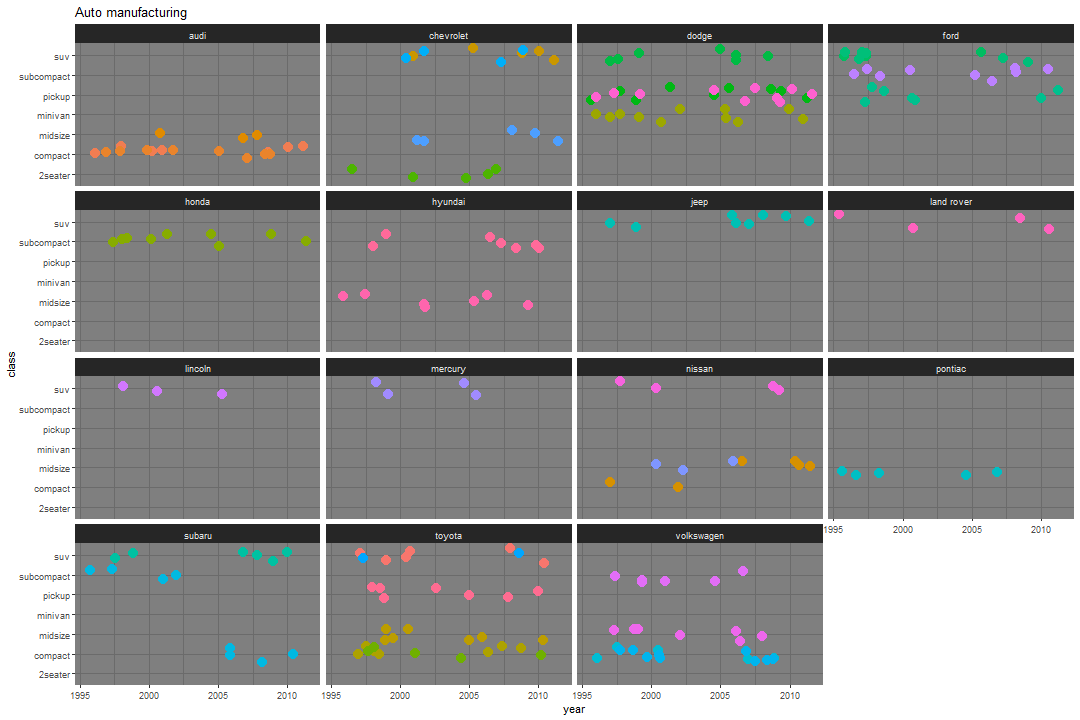
\includegraphics{5---Transformation_files/figure-latex/unnamed-chunk-35-1.pdf}

From the plot it doesn't seem to be a pattern, some days have higher
peaks but they are not from the same day (weekday = color).

The moving average on weeks does not highlight anything special, while
the monthly one (red) has a couple of spikes around christmas, first
week of january (maybe a storm?) and during summer holidays.

\begin{Shaded}
\begin{Highlighting}[]
\NormalTok{weekday\_cancelled }\OtherTok{\textless{}{-}}\NormalTok{ flights }\SpecialCharTok{\%\textgreater{}\%} 
  \FunctionTok{group\_by}\NormalTok{( year, month, day ) }\SpecialCharTok{\%\textgreater{}\%} 
  \FunctionTok{mutate}\NormalTok{( }\AttributeTok{date =} \FunctionTok{ISOdate}\NormalTok{(year, month, day),}
          \AttributeTok{weekday =} \FunctionTok{weekdays}\NormalTok{(date) ) }\SpecialCharTok{\%\textgreater{}\%} 
  \FunctionTok{group\_by}\NormalTok{(weekday) }\SpecialCharTok{\%\textgreater{}\%} 
  \FunctionTok{summarize}\NormalTok{( }\AttributeTok{prop =} \FunctionTok{mean}\NormalTok{( }\FunctionTok{is.na}\NormalTok{(arr\_delay) )) }\SpecialCharTok{\%\textgreater{}\%} 
  \FunctionTok{arrange}\NormalTok{(}\FunctionTok{desc}\NormalTok{(prop))}

\NormalTok{weekday\_cancelled}
\end{Highlighting}
\end{Shaded}

\begin{verbatim}
## # A tibble: 7 x 2
##   weekday     prop
##   <chr>      <dbl>
## 1 giovedì   0.0353
## 2 venerdì   0.0353
## 3 mercoledì 0.0285
## 4 lunedì    0.0274
## 5 martedì   0.0255
## 6 sabato    0.0239
## 7 domenica  0.0184
\end{verbatim}

The table highlights some differences but we can not discriminate the
impact of outliers (e.g.~the day where 60\% of flights got cancelled for
saturdays and fridays)

\begin{Shaded}
\begin{Highlighting}[]
\FunctionTok{ggplot}\NormalTok{(prop\_cancelled, }\AttributeTok{mapping =} \FunctionTok{aes}\NormalTok{( }\AttributeTok{x =}\NormalTok{ avg\_delay, }\AttributeTok{y =}\NormalTok{ prop)) }\SpecialCharTok{+}
  \FunctionTok{geom\_smooth}\NormalTok{()}
\end{Highlighting}
\end{Shaded}

\begin{verbatim}
## `geom_smooth()` using method = 'loess' and formula 'y ~ x'
\end{verbatim}

\includegraphics{5---Transformation_files/figure-latex/unnamed-chunk-37-1.pdf}

For avg\_delay greater than 30 min it seems to be a linear correlation.
A few outliers are visible in the geom\_point plot

\begin{enumerate}
\def\labelenumi{\arabic{enumi}.}
\tightlist
\item
  Which carrier has the worst delays? Challenge: can you disentangle the
  effects of bad airports vs.~bad carriers? Why/why not? (Hint: think
  about
  \texttt{flights\ \%\textgreater{}\%\ group\_by(carrier,\ dest)\ \%\textgreater{}\%\ summarise(n())})
\end{enumerate}

\begin{Shaded}
\begin{Highlighting}[]
\NormalTok{cd\_delays }\OtherTok{\textless{}{-}}\NormalTok{ flights }\SpecialCharTok{\%\textgreater{}\%} 
  \FunctionTok{group\_by}\NormalTok{(carrier, dest) }\SpecialCharTok{\%\textgreater{}\%} 
  \FunctionTok{summarise}\NormalTok{( }\AttributeTok{total\_delay =} \FunctionTok{sum}\NormalTok{( dep\_delay[dep\_delay }\SpecialCharTok{\textgreater{}} \DecValTok{0}\NormalTok{], }\AttributeTok{na.rm=}\ConstantTok{TRUE}\NormalTok{) )}
\end{Highlighting}
\end{Shaded}

\begin{verbatim}
## `summarise()` has grouped output by 'carrier'. You can override using the `.groups` argument.
\end{verbatim}

\begin{Shaded}
\begin{Highlighting}[]
\FunctionTok{ggplot}\NormalTok{(cd\_delays,}
       \AttributeTok{mapping =} \FunctionTok{aes}\NormalTok{( }\AttributeTok{x =} \FunctionTok{reorder}\NormalTok{(dest,total\_delay), }
                      \AttributeTok{y =} \FunctionTok{reorder}\NormalTok{(carrier, total\_delay),}
                      \AttributeTok{size =} \FunctionTok{log2}\NormalTok{(total\_delay),}
                      \AttributeTok{color =} \FunctionTok{log2}\NormalTok{(total\_delay))) }\SpecialCharTok{+}
  \FunctionTok{geom\_point}\NormalTok{() }\SpecialCharTok{+}
  \FunctionTok{scale\_color\_distiller}\NormalTok{(}\AttributeTok{palette=}\StringTok{"RdYlGn"}\NormalTok{) }\SpecialCharTok{+}
  \FunctionTok{coord\_flip}\NormalTok{()}
\end{Highlighting}
\end{Shaded}

\begin{verbatim}
## Warning in sqrt(x): Si è prodotto un NaN
\end{verbatim}

\begin{verbatim}
## Warning: Removed 22 rows containing missing values (geom_point).
\end{verbatim}

\includegraphics{5---Transformation_files/figure-latex/unnamed-chunk-38-1.pdf}

\begin{Shaded}
\begin{Highlighting}[]
\FunctionTok{ggplot}\NormalTok{(cd\_delays,}
       \AttributeTok{mapping =} \FunctionTok{aes}\NormalTok{( }\AttributeTok{x =} \FunctionTok{reorder}\NormalTok{(dest,total\_delay), }
                      \AttributeTok{y =} \FunctionTok{reorder}\NormalTok{(carrier, total\_delay),}
                      \AttributeTok{fill =} \FunctionTok{log2}\NormalTok{(total\_delay))) }\SpecialCharTok{+}
  \FunctionTok{geom\_tile}\NormalTok{() }\SpecialCharTok{+}
  \FunctionTok{scale\_fill\_distiller}\NormalTok{(}\AttributeTok{palette=}\StringTok{"RdYlGn"}\NormalTok{) }\SpecialCharTok{+}
  \FunctionTok{coord\_flip}\NormalTok{()}
\end{Highlighting}
\end{Shaded}

\includegraphics{5---Transformation_files/figure-latex/unnamed-chunk-39-1.pdf}

From this chart it seems that arr\_delays greatly depend on the company
rather than the departure airport (arrival airport does not seem a
plausible hypothesis).

\begin{enumerate}
\def\labelenumi{\arabic{enumi}.}
\tightlist
\item
  What does the \texttt{sort} argument to \texttt{count()} do. When
  might you use it?
\end{enumerate}

If TRUE, will show the largest groups at the top. Useful not to write
arrange(that variable)

\hypertarget{exercises-5}{%
\subsubsection{Exercises}\label{exercises-5}}

\begin{enumerate}
\def\labelenumi{\arabic{enumi}.}
\item
  Refer back to the lists of useful mutate and filtering functions.
  Describe how each operation changes when you combine it with grouping.
\item
  Which plane (\texttt{tailnum}) has the worst on-time record?
\end{enumerate}

\begin{Shaded}
\begin{Highlighting}[]
\NormalTok{delay\_chart }\OtherTok{\textless{}{-}}\NormalTok{ flights }\SpecialCharTok{\%\textgreater{}\%} 
  \FunctionTok{select}\NormalTok{(tailnum, arr\_delay) }\SpecialCharTok{\%\textgreater{}\%} 
  \FunctionTok{group\_by}\NormalTok{(tailnum) }\SpecialCharTok{\%\textgreater{}\%}
  \FunctionTok{summarise}\NormalTok{( }\AttributeTok{total\_flights =} \FunctionTok{n}\NormalTok{(),}
             \AttributeTok{on\_time =}\NormalTok{ ( }\FunctionTok{sum}\NormalTok{( arr\_delay }\SpecialCharTok{\textgreater{}} \DecValTok{0}\NormalTok{, }\AttributeTok{na.rm =} \ConstantTok{TRUE}\NormalTok{ ) }\SpecialCharTok{+}
                         \FunctionTok{sum}\NormalTok{( }\FunctionTok{is.na}\NormalTok{(arr\_delay) ) }
\NormalTok{                       ) }\SpecialCharTok{/} \FunctionTok{length}\NormalTok{(arr\_delay) ) }\SpecialCharTok{\%\textgreater{}\%}
  \FunctionTok{filter}\NormalTok{( }\SpecialCharTok{!}\FunctionTok{is.na}\NormalTok{(tailnum)) }\SpecialCharTok{\%\textgreater{}\%} 
  \FunctionTok{arrange}\NormalTok{(on\_time)}

\NormalTok{delay\_chart[}\DecValTok{1}\SpecialCharTok{:}\DecValTok{10}\NormalTok{,] }\CommentTok{\# print worst 10 flights}
\end{Highlighting}
\end{Shaded}

\begin{verbatim}
## # A tibble: 10 x 3
##    tailnum total_flights on_time
##    <chr>           <int>   <dbl>
##  1 N137DL              1       0
##  2 N14628              1       0
##  3 N1607B              3       0
##  4 N1608               3       0
##  5 N1610D              2       0
##  6 N206UA              1       0
##  7 N20904              2       0
##  8 N228UA              1       0
##  9 N27901              1       0
## 10 N306AS              1       0
\end{verbatim}

\begin{Shaded}
\begin{Highlighting}[]
\FunctionTok{ggplot}\NormalTok{(delay\_chart, }\AttributeTok{mapping =} \FunctionTok{aes}\NormalTok{(}\AttributeTok{x =}\NormalTok{ on\_time)) }\SpecialCharTok{+}
    \FunctionTok{geom\_density}\NormalTok{() }
\end{Highlighting}
\end{Shaded}

\includegraphics{5---Transformation_files/figure-latex/unnamed-chunk-41-1.pdf}

\begin{Shaded}
\begin{Highlighting}[]
\FunctionTok{ggplot}\NormalTok{(delay\_chart, }\AttributeTok{mapping =} \FunctionTok{aes}\NormalTok{(}\AttributeTok{x =}\NormalTok{ total\_flights)) }\SpecialCharTok{+}
    \FunctionTok{geom\_density}\NormalTok{()}
\end{Highlighting}
\end{Shaded}

\includegraphics{5---Transformation_files/figure-latex/unnamed-chunk-42-1.pdf}

The problem with the worst flights is that maybe they have flown only
few times, so they are maybe unlucky instead of chronically delayed.

\begin{Shaded}
\begin{Highlighting}[]
\FunctionTok{ggplot}\NormalTok{(delay\_chart, }\AttributeTok{mapping =} \FunctionTok{aes}\NormalTok{(}\AttributeTok{x =}\NormalTok{ on\_time, }\AttributeTok{y =}\NormalTok{ total\_flights)) }\SpecialCharTok{+}
  \FunctionTok{geom\_density2d}\NormalTok{()}
\end{Highlighting}
\end{Shaded}

\includegraphics{5---Transformation_files/figure-latex/unnamed-chunk-43-1.pdf}

\begin{Shaded}
\begin{Highlighting}[]
\FunctionTok{ggplot}\NormalTok{(}\FunctionTok{filter}\NormalTok{(delay\_chart, total\_flights }\SpecialCharTok{\textgreater{}} \DecValTok{20}\NormalTok{), }\AttributeTok{mapping =} \FunctionTok{aes}\NormalTok{(}\AttributeTok{x =}\NormalTok{ on\_time)) }\SpecialCharTok{+}
    \FunctionTok{geom\_density}\NormalTok{() }
\end{Highlighting}
\end{Shaded}

\includegraphics{5---Transformation_files/figure-latex/unnamed-chunk-44-1.pdf}

\begin{Shaded}
\begin{Highlighting}[]
\CommentTok{\# cancel low flights noise}
\NormalTok{delay\_chart\_filtered }\OtherTok{\textless{}{-}} \FunctionTok{filter}\NormalTok{(delay\_chart, total\_flights }\SpecialCharTok{\textgreater{}} \DecValTok{20}\NormalTok{)}

\CommentTok{\# fit a beta distribution (probility of probability)}
\CommentTok{\# m \textless{}{-} fitdistr(delay\_chart\_filtered$on\_time, \#MASS package}
\CommentTok{\#               dbeta, }
\CommentTok{\#               start = list(shape1 = 1, shape2 = 10)) }
\NormalTok{m }\OtherTok{\textless{}{-}}\NormalTok{ fitdistrplus}\SpecialCharTok{::}\FunctionTok{fitdist}\NormalTok{(delay\_chart\_filtered}\SpecialCharTok{$}\NormalTok{on\_time, }\StringTok{"beta"}\NormalTok{)}

\CommentTok{\#save parameters}
\NormalTok{x  }\OtherTok{\textless{}{-}}\FunctionTok{seq}\NormalTok{(}\DecValTok{0}\NormalTok{,}\DecValTok{1}\NormalTok{,}\AttributeTok{length=} \FunctionTok{dim}\NormalTok{(delay\_chart\_filtered)[}\DecValTok{1}\NormalTok{] )}
\NormalTok{alpha0 }\OtherTok{\textless{}{-}}\NormalTok{ m}\SpecialCharTok{$}\NormalTok{estimate[}\DecValTok{1}\NormalTok{]}
\NormalTok{beta0  }\OtherTok{\textless{}{-}}\NormalTok{ m}\SpecialCharTok{$}\NormalTok{estimate[}\DecValTok{2}\NormalTok{]}
\NormalTok{db }\OtherTok{\textless{}{-}} \FunctionTok{dbeta}\NormalTok{(x, alpha0, beta0)}

\FunctionTok{ggplot}\NormalTok{(delay\_chart\_filtered, }\AttributeTok{mapping =} \FunctionTok{aes}\NormalTok{(}\AttributeTok{x =}\NormalTok{ on\_time)) }\SpecialCharTok{+}
    \FunctionTok{geom\_density}\NormalTok{() }\SpecialCharTok{+}
    \FunctionTok{geom\_line}\NormalTok{(}\FunctionTok{aes}\NormalTok{(x,db), }\AttributeTok{color=}\StringTok{"red"}\NormalTok{)}
\end{Highlighting}
\end{Shaded}

\includegraphics{5---Transformation_files/figure-latex/unnamed-chunk-44-2.pdf}

Now er can update our priors

\begin{Shaded}
\begin{Highlighting}[]
\NormalTok{delay\_chart }\OtherTok{\textless{}{-}}\NormalTok{ delay\_chart }\SpecialCharTok{\%\textgreater{}\%} 
  \FunctionTok{mutate}\NormalTok{( }\AttributeTok{true\_on\_time =}\NormalTok{ (on\_time }\SpecialCharTok{*}\NormalTok{ total\_flights }\SpecialCharTok{+}\NormalTok{ alpha0) }
                         \SpecialCharTok{/}\NormalTok{ (total\_flights }\SpecialCharTok{+}\NormalTok{ alpha0 }\SpecialCharTok{+}\NormalTok{ beta0 ) ) }\SpecialCharTok{\%\textgreater{}\%} 
  \FunctionTok{arrange}\NormalTok{(true\_on\_time)}
  
\NormalTok{delay\_chart[}\DecValTok{1}\SpecialCharTok{:}\DecValTok{10}\NormalTok{,]}
\end{Highlighting}
\end{Shaded}

\begin{verbatim}
## # A tibble: 10 x 4
##    tailnum total_flights on_time true_on_time
##    <chr>           <int>   <dbl>        <dbl>
##  1 N854VA             87   0.161        0.218
##  2 N3753             130   0.185        0.222
##  3 N363NB             86   0.174        0.229
##  4 N548AA             49   0.143        0.235
##  5 N4YNAA             70   0.171        0.236
##  6 N3772H            157   0.210        0.238
##  7 N553AA             52   0.154        0.239
##  8 N847VA             91   0.198        0.245
##  9 N117UW             46   0.152        0.245
## 10 N839VA            127   0.213        0.246
\end{verbatim}

Under the assumption that all flights are drawn from the same
distribution. This result was obtained by replicating tutorial on
\url{http://varianceexplained.org/r/empirical_bayes_baseball/}

\begin{enumerate}
\def\labelenumi{\arabic{enumi}.}
\tightlist
\item
  What time of day should you fly if you want to avoid delays as much as
  possible?
\end{enumerate}

\begin{Shaded}
\begin{Highlighting}[]
\FunctionTok{ggplot}\NormalTok{(flights) }\SpecialCharTok{+}
  \FunctionTok{geom\_density}\NormalTok{(}\FunctionTok{aes}\NormalTok{(dep\_time\_min))}
\end{Highlighting}
\end{Shaded}

\begin{verbatim}
## Warning: Removed 8255 rows containing non-finite values (stat_density).
\end{verbatim}

\includegraphics{5---Transformation_files/figure-latex/unnamed-chunk-46-1.pdf}

\begin{Shaded}
\begin{Highlighting}[]
\NormalTok{hour\_delay }\OtherTok{\textless{}{-}}\NormalTok{ flights }\SpecialCharTok{\%\textgreater{}\%} 
    \FunctionTok{group\_by}\NormalTok{(hour) }\SpecialCharTok{\%\textgreater{}\%} 
    \FunctionTok{summarise}\NormalTok{( }\AttributeTok{prob\_delay =} \FunctionTok{mean}\NormalTok{( arr\_delay }\SpecialCharTok{\textless{}=} \DecValTok{0}\NormalTok{, }\AttributeTok{na.rm =} \ConstantTok{TRUE}\NormalTok{),}
               \AttributeTok{total\_flights =} \FunctionTok{n}\NormalTok{() ) }\SpecialCharTok{\%\textgreater{}\%} 
    \FunctionTok{arrange}\NormalTok{(hour)}

\FunctionTok{ggplot}\NormalTok{(hour\_delay) }\SpecialCharTok{+}
  \FunctionTok{geom\_point}\NormalTok{( }\FunctionTok{aes}\NormalTok{(hour, prob\_delay, }\AttributeTok{color =}\NormalTok{ total\_flights }\SpecialCharTok{\textgreater{}} \DecValTok{2000}\NormalTok{) ) }\SpecialCharTok{+}
  \FunctionTok{ggtitle}\NormalTok{(}\StringTok{"probability( arr\_delay \textless{}= 0 )"}\NormalTok{)}
\end{Highlighting}
\end{Shaded}

\begin{verbatim}
## Warning: Removed 1 rows containing missing values (geom_point).
\end{verbatim}

\includegraphics{5---Transformation_files/figure-latex/unnamed-chunk-47-1.pdf}

The probability of an on time flights decreases as the hours in the day
pass

\begin{enumerate}
\def\labelenumi{\arabic{enumi}.}
\tightlist
\item
  For each destination, compute the total minutes of delay. For each
  flight, compute the proportion of the total delay for its destination.
\end{enumerate}

\begin{Shaded}
\begin{Highlighting}[]
\NormalTok{flights }\SpecialCharTok{\%\textgreater{}\%} 
  \FunctionTok{group\_by}\NormalTok{(dest) }\SpecialCharTok{\%\textgreater{}\%} 
  \FunctionTok{summarise}\NormalTok{( }\AttributeTok{tota\_delay =} \FunctionTok{sum}\NormalTok{(arr\_delay }\SpecialCharTok{*}\NormalTok{ (arr\_delay }\SpecialCharTok{\textgreater{}} \DecValTok{0}\NormalTok{), }
                              \AttributeTok{na.rm =} \ConstantTok{TRUE}\NormalTok{),}
          \AttributeTok{total\_flights =} \FunctionTok{n}\NormalTok{())}
\end{Highlighting}
\end{Shaded}

\begin{verbatim}
## # A tibble: 105 x 3
##    dest  tota_delay total_flights
##  * <chr>      <dbl>         <int>
##  1 ABQ         4487           254
##  2 ACK         2974           265
##  3 ALB         9580           439
##  4 ANC           62             8
##  5 ATL       300299         17215
##  6 AUS        39940          2439
##  7 AVL         3671           275
##  8 BDL         6953           443
##  9 BGR         6940           375
## 10 BHM         7267           297
## # ... with 95 more rows
\end{verbatim}

\begin{Shaded}
\begin{Highlighting}[]
\NormalTok{delay\_prop\_flights }\OtherTok{\textless{}{-}}\NormalTok{ flights }\SpecialCharTok{\%\textgreater{}\%} 
  \FunctionTok{group\_by}\NormalTok{(dest) }\SpecialCharTok{\%\textgreater{}\%} 
  \FunctionTok{mutate}\NormalTok{( }\AttributeTok{total\_delay =} \FunctionTok{sum}\NormalTok{(arr\_delay }\SpecialCharTok{*}\NormalTok{ (arr\_delay }\SpecialCharTok{\textgreater{}} \DecValTok{0}\NormalTok{), }
                              \AttributeTok{na.rm =} \ConstantTok{TRUE}\NormalTok{),}
          \AttributeTok{total\_flights =} \FunctionTok{n}\NormalTok{()) }\SpecialCharTok{\%\textgreater{}\%} 
  \FunctionTok{ungroup}\NormalTok{() }\SpecialCharTok{\%\textgreater{}\%} 
  \FunctionTok{group\_by}\NormalTok{(flight) }\SpecialCharTok{\%\textgreater{}\%} 
  \FunctionTok{summarise}\NormalTok{( }\AttributeTok{delay\_proportion =}\NormalTok{ (arr\_delay }\SpecialCharTok{\textgreater{}} \DecValTok{0}\NormalTok{) }\SpecialCharTok{*}\NormalTok{ (arr\_delay }\SpecialCharTok{/}\NormalTok{ total\_delay) )}
\end{Highlighting}
\end{Shaded}

\begin{verbatim}
## `summarise()` has grouped output by 'flight'. You can override using the `.groups` argument.
\end{verbatim}

\begin{Shaded}
\begin{Highlighting}[]
\NormalTok{delay\_prop\_flights }
\end{Highlighting}
\end{Shaded}

\begin{verbatim}
## # A tibble: 336,776 x 2
## # Groups:   flight [3,844]
##    flight delay_proportion
##     <int>            <dbl>
##  1      1       0.0000295 
##  2      1       0.000143  
##  3      1       0.0000246 
##  4      1       0.000118  
##  5      1       0         
##  6      1       0.000222  
##  7      1       0         
##  8      1       0.00000987
##  9      1       0         
## 10      1       0         
## # ... with 336,766 more rows
\end{verbatim}

\begin{enumerate}
\def\labelenumi{\arabic{enumi}.}
\tightlist
\item
  Delays are typically temporally correlated: even once the problem that
  caused the initial delay has been resolved, later flights are delayed
  to allow earlier flights to leave. Using \texttt{lag()}, explore how
  the delay of a flight is related to the delay of the immediately
  preceding flight.
\end{enumerate}

\begin{Shaded}
\begin{Highlighting}[]
\NormalTok{lag\_flights }\OtherTok{\textless{}{-}}\NormalTok{ flights }\SpecialCharTok{\%\textgreater{}\%} 
  \FunctionTok{group\_by}\NormalTok{(origin, year, month, day) }\SpecialCharTok{\%\textgreater{}\%} 
  \FunctionTok{summarise}\NormalTok{( }\AttributeTok{diff =} \FunctionTok{lag}\NormalTok{(dep\_delay) }\SpecialCharTok{{-}}\NormalTok{ dep\_delay,}
             \AttributeTok{q25 =} \FunctionTok{quantile}\NormalTok{(diff, }\FloatTok{0.25}\NormalTok{, }\AttributeTok{na.rm =} \ConstantTok{TRUE}\NormalTok{),}
             \AttributeTok{q50 =} \FunctionTok{quantile}\NormalTok{(diff, }\FloatTok{0.25}\NormalTok{, }\AttributeTok{na.rm =} \ConstantTok{TRUE}\NormalTok{),}
             \AttributeTok{q75 =} \FunctionTok{quantile}\NormalTok{(diff, }\FloatTok{0.25}\NormalTok{, }\AttributeTok{na.rm =} \ConstantTok{TRUE}\NormalTok{),}
             \AttributeTok{mean =} \FunctionTok{mean}\NormalTok{(diff, }\AttributeTok{na.rm =} \ConstantTok{TRUE}\NormalTok{) )}

\CommentTok{\# ok this does not work}
\end{Highlighting}
\end{Shaded}

\begin{enumerate}
\def\labelenumi{\arabic{enumi}.}
\tightlist
\item
  Look at each destination. Can you find flights that are suspiciously
  fast? (i.e.~flights that represent a potential data entry error).
  Compute the air time of a flight relative to the shortest flight to
  that destination. Which flights were most delayed in the air?
\end{enumerate}

\begin{Shaded}
\begin{Highlighting}[]
\NormalTok{flights }\SpecialCharTok{\%\textgreater{}\%} 
  \FunctionTok{group\_by}\NormalTok{(dest) }\SpecialCharTok{\%\textgreater{}\%} 
  \FunctionTok{mutate}\NormalTok{( }\AttributeTok{mph =}\NormalTok{  (distance}\SpecialCharTok{*}\DecValTok{60}\NormalTok{) }\SpecialCharTok{/}\NormalTok{ air\_time ) }\SpecialCharTok{\%\textgreater{}\%} 
  \FunctionTok{summarise}\NormalTok{( }\AttributeTok{max\_mph =} \FunctionTok{max}\NormalTok{(mph, }\AttributeTok{na.rm =} \ConstantTok{TRUE}\NormalTok{) ) }\SpecialCharTok{\%\textgreater{}\%} 
  \FunctionTok{arrange}\NormalTok{( }\FunctionTok{desc}\NormalTok{(max\_mph) )}
\end{Highlighting}
\end{Shaded}

\begin{verbatim}
## Warning in max(mph, na.rm = TRUE): no non-missing arguments to max; returning -
## Inf
\end{verbatim}

\begin{verbatim}
## # A tibble: 105 x 2
##    dest  max_mph
##    <chr>   <dbl>
##  1 ATL      703.
##  2 MSP      650.
##  3 GSP      648 
##  4 BNA      641.
##  5 PBI      591.
##  6 SJU      564 
##  7 STT      556.
##  8 CVG      551.
##  9 BQN      550.
## 10 PSE      542.
## # ... with 95 more rows
\end{verbatim}

All velocities seem to be plausible.

Regarding the flights that got delayed the most while they were flying,
we must consider - a non delayed flights takes air\_time to travel
between two cities - a dep\_delayed flights takes air\_time to travel
and should arrive at air\_time + dep\_delay if no further delay is
accumulated - in other words, arr\_delay = air\_time + dep\_delay +
mid\_air\_delay - or mid\_air\_delay = arr\_delay - (air\_time +
dep\_delay)

To see which were delayed the most\ldots{}

\begin{Shaded}
\begin{Highlighting}[]
\NormalTok{flights }\SpecialCharTok{\%\textgreater{}\%} 
  \FunctionTok{mutate}\NormalTok{( }\AttributeTok{mid\_air\_delay =}\NormalTok{ arr\_delay }\SpecialCharTok{{-}}\NormalTok{ (air\_time }\SpecialCharTok{+}\NormalTok{ dep\_delay) ) }\SpecialCharTok{\%\textgreater{}\%} 
  \FunctionTok{group\_by}\NormalTok{(flight) }\SpecialCharTok{\%\textgreater{}\%} 
  \FunctionTok{summarise}\NormalTok{( }\AttributeTok{max\_mid\_air\_delay =} \FunctionTok{max}\NormalTok{(mid\_air\_delay)) }\SpecialCharTok{\%\textgreater{}\%} 
  \FunctionTok{arrange}\NormalTok{( }\FunctionTok{desc}\NormalTok{(max\_mid\_air\_delay))}
\end{Highlighting}
\end{Shaded}

\begin{verbatim}
## # A tibble: 3,844 x 2
##    flight max_mid_air_delay
##     <int>             <dbl>
##  1   2402                64
##  2     34                63
##  3   5667                47
##  4   2944                39
##  5   3289                34
##  6   5978                33
##  7    477                32
##  8    588                32
##  9   5329                27
## 10   1028                26
## # ... with 3,834 more rows
\end{verbatim}

\begin{enumerate}
\def\labelenumi{\arabic{enumi}.}
\tightlist
\item
  Find all destinations that are flown by at least two carriers. Use
  that information to rank the carriers.
\end{enumerate}

\begin{Shaded}
\begin{Highlighting}[]
\NormalTok{flights }\SpecialCharTok{\%\textgreater{}\%} 
  \FunctionTok{group\_by}\NormalTok{(dest) }\SpecialCharTok{\%\textgreater{}\%} 
  \FunctionTok{mutate}\NormalTok{( }\AttributeTok{more\_than\_1 =} \FunctionTok{n\_distinct}\NormalTok{(carrier) }\SpecialCharTok{\textgreater{}=} \DecValTok{2}\NormalTok{ ) }\SpecialCharTok{\%\textgreater{}\%} 
  \FunctionTok{ungroup}\NormalTok{() }\SpecialCharTok{\%\textgreater{}\%} 
  \FunctionTok{group\_by}\NormalTok{(carrier, dest) }\CommentTok{\# \%\textgreater{}\%  don\textquotesingle{}t understand}
\end{Highlighting}
\end{Shaded}

\begin{enumerate}
\def\labelenumi{\arabic{enumi}.}
\tightlist
\item
  For each plane, count the number of flights before the first delay of
  greater than 1 hour.
\end{enumerate}

\begin{Shaded}
\begin{Highlighting}[]
\NormalTok{flights }\SpecialCharTok{\%\textgreater{}\%} 
  \FunctionTok{select}\NormalTok{(tailnum, time\_hour, dep\_delay) }\SpecialCharTok{\%\textgreater{}\%} 
  \FunctionTok{group\_by}\NormalTok{(tailnum) }\SpecialCharTok{\%\textgreater{}\%} 
  \FunctionTok{filter}\NormalTok{( dep\_delay }\SpecialCharTok{\textgreater{}} \DecValTok{60}\NormalTok{ ) }\SpecialCharTok{\%\textgreater{}\%} 
  \FunctionTok{filter}\NormalTok{( }\FunctionTok{rank}\NormalTok{(time\_hour) }\SpecialCharTok{==} \DecValTok{1}\NormalTok{)}
\end{Highlighting}
\end{Shaded}

\begin{verbatim}
## # A tibble: 3,360 x 3
## # Groups:   tailnum [3,360]
##    tailnum time_hour           dep_delay
##    <chr>   <dttm>                  <dbl>
##  1 N531MQ  2013-01-01 06:00:00       101
##  2 N3GVAA  2013-01-01 07:00:00        71
##  3 N942MQ  2013-01-01 18:00:00       853
##  4 N534UA  2013-01-01 07:00:00       144
##  5 N76502  2013-01-01 09:00:00       134
##  6 N16561  2013-01-01 09:00:00        96
##  7 N542MQ  2013-01-01 11:00:00        71
##  8 N636JB  2013-01-01 12:00:00        77
##  9 N748EV  2013-01-01 12:00:00        70
## 10 N17984  2013-01-01 13:00:00       115
## # ... with 3,350 more rows
\end{verbatim}

\end{document}
